\documentclass[onecolumn]{revtex4-2}
\usepackage{amsmath}
\usepackage{graphicx}
\renewcommand{\vec}[1]{\boldsymbol{#1}}
\begin{document}
\title{Summary of results}
%\author{Christopher K\"orber}
\maketitle

\section{Operator definitions}

All of the results are very preliminary and I need to run further cross-checks.
For now, these plots rather indicate the $q^2$ scaling.

\subsection{One-Nucleon Elements}
Kinematics for single-nucleon system
\begin{equation}
    N(\vec p_1) + J(\vec q) \to N(\vec p_1')
\end{equation}

Operator definitions
\begin{align}
    \mathcal{O}_{1N}^{(1)}
    &=
    1
    \,\\
    \mathcal{O}_{1N}^{(DF)}
    &=
    \frac{k^2}{8 m_N^2}
    \,\\
    \mathcal{O}_{1N}^{(SO)}
    &=
    \frac{i}{4 m_N^2} \vec \sigma_1 \cdot (\vec q \times (\vec p_1 + \vec p_1'))
    =
    \frac{i}{2 m_N^2} \vec \sigma_1 \cdot (\vec q \times \vec p_1 )
\end{align}
where $\vec \sigma_1$ is the Pauli (spin) matrix of the first nucleon.

\subsection{Two-Nucleon Elements}

Kinematics for two-nucleon system
\begin{equation}
    N(\vec p_1) + N(\vec p_1) + J(\vec q) \to N(\vec p_1') +N(\vec p_2')
\end{equation}

Operator definitions
\begin{align}
    \mathcal{O}_{2N}^{(1\pi_1)}
    &=
    \frac{-3 g_A^2}{16 F_\pi^2 m_N}
    \frac{(\vec \sigma_1 \cdot \vec q)(\vec \sigma_1 \cdot \vec q_2)}{\vec q_2^2 + M_\pi^2}
    + (1 \leftrightarrow 2)
    \,\\
    \mathcal{O}_{2N}^{(1\pi_2)}
    &=
    \frac{-3 g_A^2}{16 F_\pi^2 m_N}
    \frac{(\vec \sigma_1 \cdot \vec q_2)(\vec \sigma_2 \cdot \vec q_2)(\vec q_2 \cdot \vec k)}{\vec q_2^2 + M_\pi^2}
    + (1 \leftrightarrow 2)
\end{align}
with $\vec q_1 = \vec p_1' - \vec p_1$ and $\vec q_2 = \vec p_2' - \vec p_2$ and
\begin{align}
    \mathcal{O}_{2N}^{(A)}
    &=
    2 \vec q^2 \to 2 F_1(\vec p_{12}, \vec p_{12}', \vec q)
    \, , \\
    \mathcal{O}_{2N}^{(B)}
    &=
    2 \vec q^2 (\vec \sigma_1 \cdot \vec \sigma_2) \to 2 (\vec \sigma_1 \cdot \vec \sigma_2) F_1(\vec p_{12}, \vec p_{12}', \vec q, \Lambda)
    \, , \\
    \mathcal{O}_{2N}^{(C)}
    &=
    2 (\vec \sigma_1 \cdot \vec q)(\vec \sigma_2 \cdot \vec q) \to 2 F_2(\vec p_{12}, \vec p_{12}', \vec q, \Lambda)
\end{align}
and $\vec p_{12} = (\vec p_1 - \vec p_2)/2$

\section{Parameters}
\begin{align}
    \hbar c &= 197.327 [\mathrm{MeV} \, \mathrm{fm}]\, , &
    m_N &= 938.918 \, [\mathrm{MeV}] \, , &
    g_A &= 1.29 \, , &
    m_\pi &= 138.03 \, [\mathrm{MeV}] \, , &
    F_\pi &= 92.4 \, [\mathrm{MeV}] \, .
\end{align}

\section{Wave function}
\begin{table}[htb!]
    \caption{The following matrix elements will be evaluated for the wave function}
    \label{}
    \begin{tabular}{ll}
    nuc       &       4he \\
    potential &     chsms \\
    order     &     n4lo+ \\
    empot     &     pCoul \\
    cmpi      &  n2locmpi \\
    tnfcut    &         $3$ \\
    cut       &        $4$\\
    \end{tabular}$\quad$
    \begin{tabular}{ll}
    $n_{p_{12}} = n_{p_{34}}$ &      $28+8$ \\
    $n_{p_{3}}$       &      $44+8$ \\
    $n_{q_4} = n_q$   &      $38+6$ \\
    $\Lambda$       &       $550$\\
    $c_1$        &  $-1.23$ \\
    $c_3$        &  $-4.65$ \\
    $c_4$        &  $3.28$
    \end{tabular}
\end{table}

\section{Results}


\subsection{Two-nucleon one-pion exchange}
\begin{figure}[htb!]
    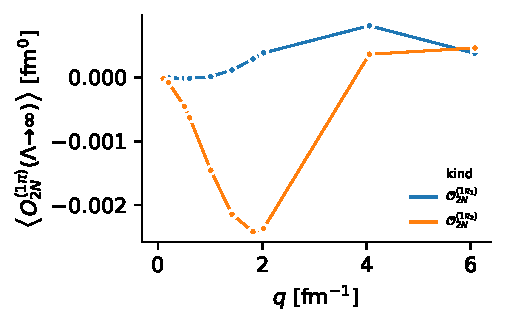
\includegraphics{figs/2n-ope.pdf}
    \caption{Differnt 2N OPE contributions.}
    \label{}
\end{figure}

\subsection{Two-nucleon contact}
\begin{figure}[htb!]
    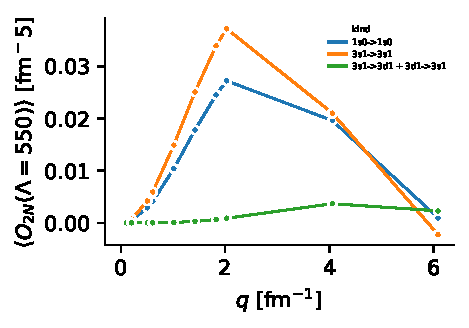
\includegraphics{figs/2n-contact.pdf}
    \caption{Differnt 2N contact contributions.}
    \label{}
\end{figure}

\end{document}
